\section{Using SSHCure} \label{sec:using_sshcure}

The SSHCure frontend consists of the following three pages:

\begin{description}
	\item [Dashboard] -- The Dashboard page shows an overview over your network with respect to SSH attacks. Besides showing a list of attacks for a selected period of time, it shows statistics on top attackers and targets.
	
	\item [Attack Details] -- The Attack Details page provides information on one specific attack, providing general attack statistics, a list of targets and an attack profile plot.
	
	\item [Host Details] -- The Host Details page lists details about a specific host, either an attacker or a target. Besides geolocation and reverse DNS information, the page lists the attacks in which the host participated as an attack and/or target.
\end{description}

The following pages contain screenshots of each of these pages, combined with a description of their contents.

\newpage

\begin{figure}[!ht]
	\centering
    	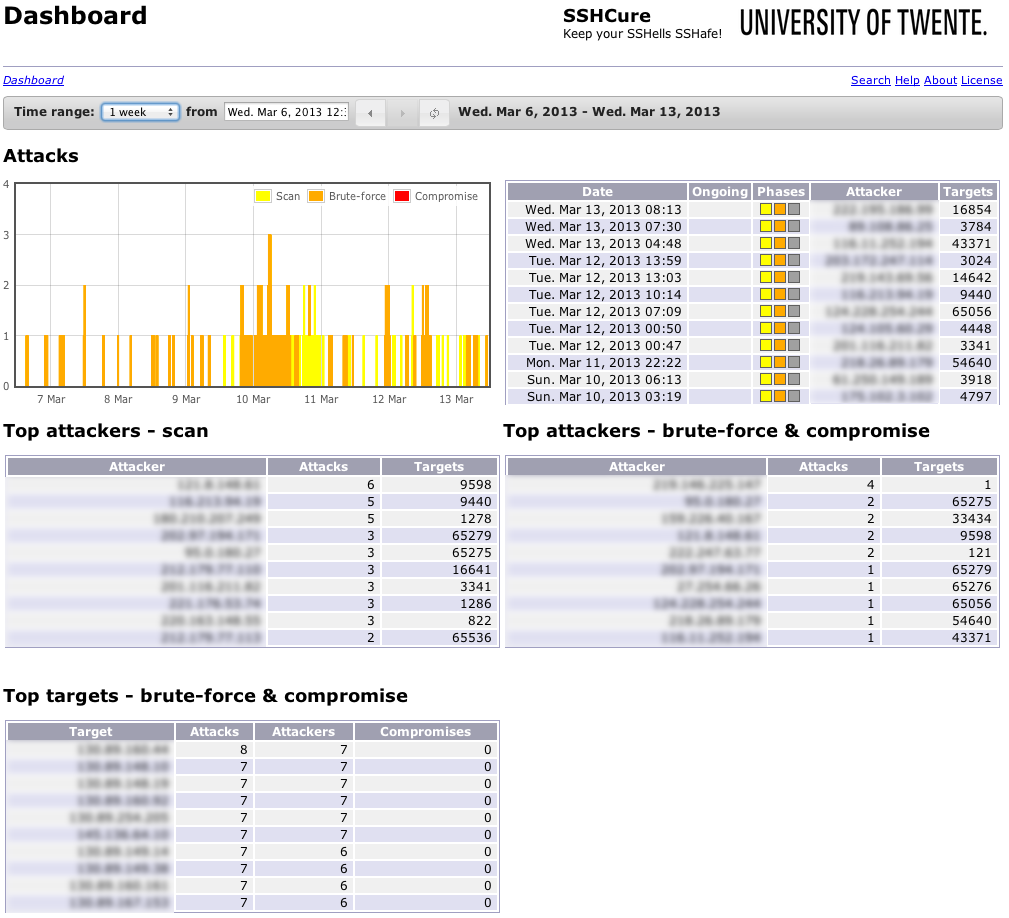
\includegraphics[width=\textwidth]{img/Screenshot_Dashboard_anonymized.png}
	\caption{SSHCure's Dashboard page}
	\label{fig:screenshot_Dashboard}
\end{figure}

At the top of the Dashboard page the time range for the page can be selected. In this screenshot, a time range of `1 week' has been selected. To the right of the time range selector a date/time selector can be found for setting the start of the time range. The following three buttons can be found next to it:

\begin{enumerate}
	\item Back -- Navigate backwards in time by the selected time range -- in the case of the screenshot `1 week'.
	\item Forward -- Navigate forward in time by the selected time range. That button has been disabled in this screenshot, as it is not possible to navigate into the future.
	\item Auto-Refresh / Now -- When the currently selected time range is the latest available, the third button can be used to enabled 'auto-refresh-'. This will update your Dashboard every five minutes, as new data becomes available to NfSen. If the currently selected time range is in the past, the last button can be used to forward to 'now'.
\end{enumerate}

The top left of the Dashboard page shows an attack history plot, where the number of attacks per attack type is shown for the selected time range. Next to it is a list of all attacks that shows all attacks during that occurred during the selected time range. The remaining lists shows statistics for the top scan attackers, top brute-force and compromise attackers and top targets.

\newpage

\begin{figure}[!ht]
	\centering
    	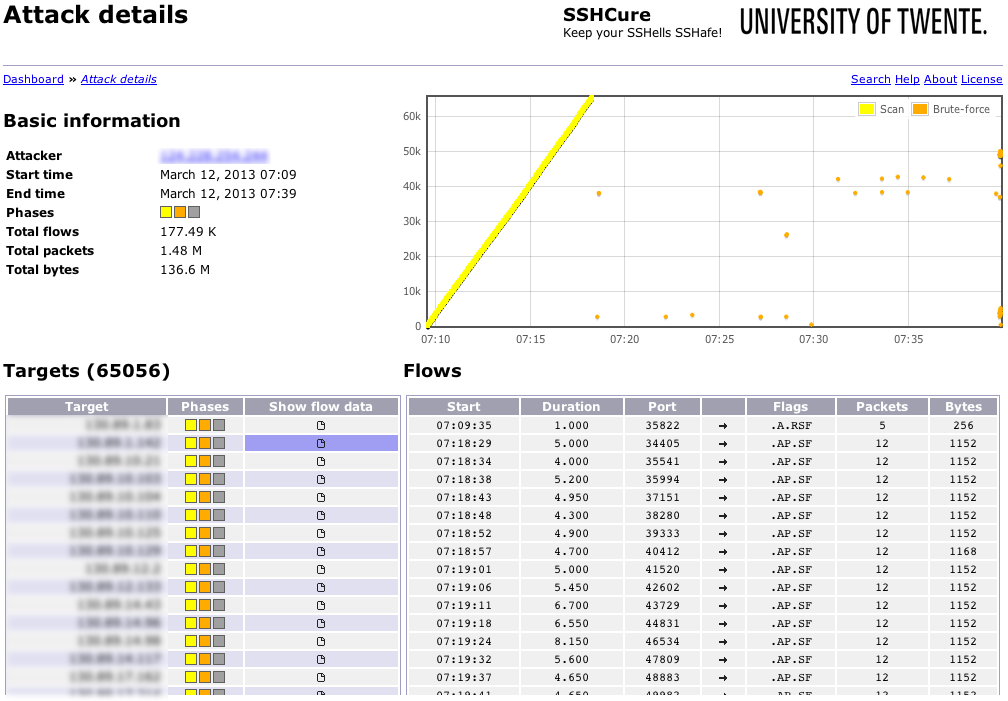
\includegraphics[width=\textwidth]{img/Screenshot_AttackDetails_anonymized.png}
	\caption{SSHCure's Attack Details page}
	\label{fig:screenshot_AttackDetails}
\end{figure}

The top left of the Attack Details page shows basic information on the selected attack, such as start and end time, the identified attack phases and statistics on the network traffic that was part of the attack. In the case of the screenshot, the attack consisted of both a scan and brute-force attempts, but no compromise (so the attack was not successful). To the right of the basic information is an attack profile plot, which shows the contacted hosts (y-axis) and the time (x-axis). It can be observed that a horizontal network scan took place from 07:10 -- 07:18, after which several individual hosts have been brute-forced by means of a dictionary attack.

At the bottom of the page a list of targets is shown. For very large attacks, not all attacks are shown\footnote{See Section~\ref{subsec:frontend_configuration} for more details.}. For each of the listed targets the corresponding flow data can be shown to the right of the targets listing. In the case of the screenshot, flow data is shown for the second target.

\newpage

\begin{figure}[!ht]
	\centering
    	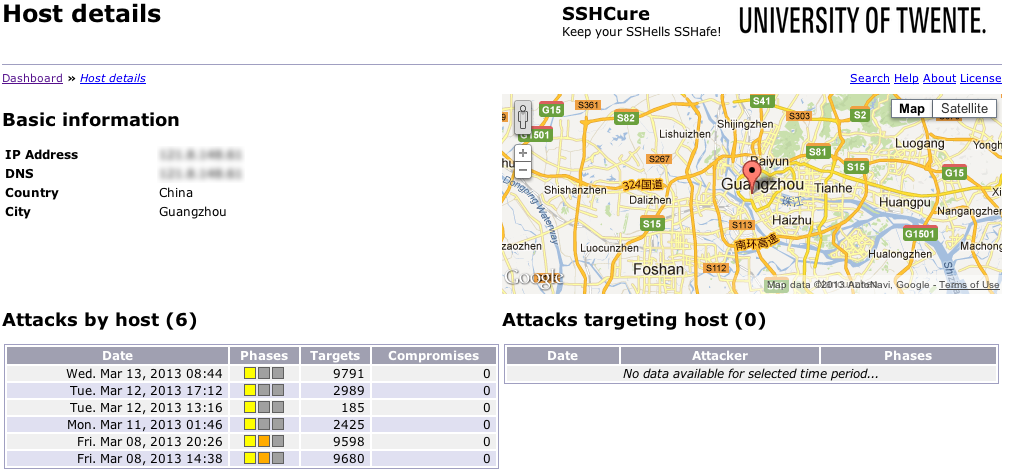
\includegraphics[width=\textwidth]{img/Screenshot_HostDetails_anonymized.png}
	\caption{SSHCure's Host Details page}
	\label{fig:screenshot_HostDetails}
\end{figure}

The third type of page within SSHCure is the Host Details page, which shows specific information on hosts (both attackers and targets). Some basic information, such as IP address, reverse DNS and geolocation information are shown at the top of the page. The bottom of the page consists of two lists: `Attacks by host' and `Attacks targeting hosts'. The first lists all attacks in which the selected host participated as an attacker. The second lists all attacks in which the selected host has been a target.
